\documentclass[conference,onecolumn]{IEEEtran}
% Readable supporting material: IEEEtran Times Roman, one column for full ledgers.
\usepackage[T1]{fontenc}
\usepackage{graphicx,microtype,amsmath,amssymb,booktabs,longtable,array,listings}
\usepackage[hidelinks]{hyperref}
\makeatletter\setlength{\@fptop}{0pt}\setlength{\@fpsep}{12pt}\makeatother
\raggedbottom
\lstset{basicstyle=\ttfamily\footnotesize,breaklines=true,columns=fullflexible,keepspaces=true,frame=single}
\title{Supporting Material for\\Fixed Geometric Health Decisions After LiDAR Degeneracy}
\author{\IEEEauthorblockN{Harshil Patel, Daksha Lingampeta, and Nisarg Vyas}}
\begin{document}\maketitle
\begin{abstract}
This supplement records the formal endpoint distinctions, exact configuration,
geometry-screen history, existing sensitivity analyses, development repeatability
and complete policy-event ledger supporting the controlled transfer study.
It typesets retained evidence; it introduces no new native runs or threshold fitting.
The independent final sampling unit is a geometry pair. There are 48 pairs,
192 native scene/backend runs, and 192 corridor policy-event rows; the latter
two counts must not be interpreted as 192 independent geometries.
\end{abstract}

\section{Evidence scope and reading map}
The main manuscript contains the primary operational definitions, fixed-policy
results and interpretation. The supporting CSV files retain full precision;
printed tables round values only for readability. The primary exports are
\path{research_paper/evidence/final_geometry_v2_results_20261012/}.
The exploratory miss diagnosis is separately recorded in
\path{final_failure_analysis_20261012/}. Its categories and example selection
were produced after the primary results and are not preregistered hypotheses.
All examples in the main paper use the existing lowest-seed selection rule.
Source hashes and the exact timeline choices are retained in the adjacent
\path{support/asset_manifest.json} and \path{support/timeline_selection.json}.
No test-set threshold, revised label, selected example or new bootstrap was
used to replace a primary result during this manuscript revision.

\section{Formal endpoint arguments}
These elementary arguments state what the measurements do and do not establish.
They are explanatory proofs, not claims of new mathematical theorems.

\subsection{Relative motion is invariant to a constant world-frame change}
Let $T(t)\in SE(3)$ map the body frame to a world frame and let a constant
$A\in SE(3)$ redefine that world frame. Then
\begin{equation}
(AT(t_a))^{-1}(AT(t_b))=T(t_a)^{-1}A^{-1}AT(t_b)
=T(t_a)^{-1}T(t_b).
\end{equation}
Thus each relative transform, and the discrepancy between estimated and reference
relative transforms in the same body-frame convention, is unchanged by a constant
left world transform. This does not prove invariance to time-varying frame errors,
incorrect extrinsics, scale changes or estimator resets. Reset-crossing windows
are explicitly unavailable. Good relative motion also does not imply small
accumulated global position error.

\subsection{A fixed geometric Hessian does not bound arbitrary bias}
Assume a linear measurement model $y=Jx^\star+b$ with $J\in\mathbb R^{m\times n}$
full column rank. The unique least-squares solution is
\begin{equation}
\widehat{x}=(J^\top J)^{-1}J^\top y
=x^\star+(J^\top J)^{-1}J^\top b.
\end{equation}
For any vector $v\in\mathbb R^n$, choose $b=Jv$. Then
$\widehat{x}-x^\star=v$, while $J^\top J$ is unchanged. Therefore a score
computed only from this Hessian cannot give an unconditional finite error bound
when $b$ is unrestricted. If instead $\lVert b\rVert\leq B$, then
$\lVert\widehat{x}-x^\star\rVert\leq B/\sigma_{\min}(J)$; the missing
assumption matters. This is a linear-model counterexample, not evidence that
this particular bias caused any native-run failure, nor a proof that geometry
has no predictive value.

\subsection{An active state need not produce a new recovery announcement}
For consecutive available decision ticks let $z_j\in\{0,1\}$ denote confirmed
health and $a_j=z_j(1-z_{j-1})$ a transition announcement. If $z_j=1$ before
reference-defined onset and remains one throughout the recovered interval,
then $a_j=0$ throughout that interval. The state overlaps recovered motion,
but no new post-onset announcement exists. This proves that a missed declaration
alone cannot establish continuously unhealthy output. Missing or reset evidence
clears confirmation; this argument applies to an uninterrupted available segment.
The online decision sees only past diagnostic records. Reference onset is
retrospective and is never an input to the state machine.

\section{Exact timing, decisions and uncertainty}
Primary motion windows have nominal non-overlapping one-second boundaries.
The nearest pose within $\pm0.05$ s is selected once per boundary, with earlier
pose on a tie; actual duration must be 0.9--1.1 s. A window passes when relative
translation error is at most 0.20 m and rotation error at most $5^\circ$.
Recovery is the first three consecutive passing post-exit windows by exit plus
20 s. Onset is the first actual window start, confirmation the third end.
A later required failed/unavailable window ends the episode at its start;
otherwise it ends at the deadline. One relapse is observed per backend.
Completed non-recoveries remain distinct from failed execution.

Decisions use a 10 Hz grid, latest same-segment record no older than 0.2 s,
and three distinct healthy source records on consecutive ticks. A newer invalid
record cannot be skipped. The minimum accepted-row count is six.
The scalar score uses a 3 m lever arm and fixed $N\,0.001$ normalization;
these are measurement-geometry conventions rather than a calibrated posterior.
The fixed Schur adaptation uses condition ratio 10 and pseudoinverse relative
rank tolerance $10^{-12}$. It does not implement DCReg's full estimator or
mitigation. Scalar thresholds are 166.16366016039856 (FAST-LIO) and
123.80876977779258 (Point-LIO), selected only on development corridor seeds
14--45. The development selection ceiling is 10\% conditional initial
false-healthy events; sensitivity is maximized and ties favor the higher threshold.

Event proportions use Wilson 95\% intervals. The paired interior-motion effect
uses each scene's median error on the predeclared central corridor region,
corridor minus matched control, then equal geometry-group weighting. Its
percentile interval uses 10,000 geometry-pair bootstrap replicates within the
four fixed groups, PCG seed 20260926 and linear quantiles. Policies on the
same geometry and timestamps within a run are not independent samples.
Detected-only median delays condition on successful declarations and must be
read with the missed-event counts.

\section{Simulator and native identities}
The simulator uses 60 s runs, a right-handed z-up frame, opaque rectangular
surfaces, 0.8 m/s nominal cruise and prescribed smooth three-dimensional motion.
LiDAR has 16 beams over $\pm15^\circ$, 360 azimuth samples and 10 Hz scans.
Range noise standard deviation is 0.01 m. IMU rate is 200 Hz with white noise
0.002 rad/s and 0.02 m/s$^2$; initial bias standard deviations are 0.003 rad/s
and 0.03 m/s$^2$. Random walks are 0.0001 rad/s/$\sqrt{\mathrm s}$ and
0.001 m/s$^2$/$\sqrt{\mathrm s}$ respectively. Floor and ceiling are at
$z=-1$ and 2 m. The pre-entry room spans $x=-12$ to 0 and the post-exit
room $x=L$ to 50 m, with sampled half-width 4.5--7.5 m.
The control adds partial positive-side baffles at $x=Li/(n+1)$,
$n=\max(4,\lceil L/(2\,\mathrm m)\rceil-1)$, spanning $y=0.65w$ to $w$ and
$z=-1$ to 1.5 m while preserving the open route. The serialized paired IMU
stream and prescribed trajectory match. Surface returns change with the baffles.

Each backend has 96 completed final runs. The identities below agree across
all 96 manifests for that backend, checked against the retained receipt hashes.
The JSON records upstream commits, binary hashes, configuration hashes and
worktree-patch hashes. A commit identifier alone is insufficient for these
instrumented builds. Historical configuration filenames include ``development''
or ``bootstrap''; receipt hashes establish their actual use in the final runs.
\lstinputlisting{support/native_build_identities.json}
\subsection{FAST-LIO configuration, verbatim}
\lstinputlisting{support/fastlio_simulation_bootstrap.yaml}
\subsection{Point-LIO configuration, verbatim}
\lstinputlisting{support/point_lio_simulation_development.yaml}

\section{Geometry screening and retained workflow history}
The original screen failed: 68 candidates yielded short/narrow 12, short/wide 10,
long/narrow 0 and long/wide 12 eligible layouts, insufficient for the planned
balanced final design. Its exact historical byte digest could not be reconciled
because the original bytes are unavailable. The retained reconciliation explicitly
records \texttt{UNRESOLVED\_ORIGINAL\_BYTES\_NOT\_AVAILABLE}; this limitation
is not silently converted into a successful provenance claim.

The revised, separately frozen geometry-only screen checked 64 candidates and
selected 12 per group, 48 total, without inspecting final estimator accuracy or
scores. Short lengths span 8--9 m, long 15--18 m; narrow half-widths 1.3--1.5 m,
wide 2.5--3.0 m. Development lengths were 9--13 m and half-widths 1.6--2.4 m.
Eligibility requires axial-normal fraction $f_c\leq0.10$ in the corridor,
$f_u\geq0.15$ in the matched control, and $f_{+5}\geq0.20$ at five seconds
past exit. These fractions screen geometry, not observed recovery.
The test population is conditional on this screen; it is not every possible corridor.
Table rows below include unsuccessful and unused candidates.
\begingroup\footnotesize
\begin{longtable}{@{}llrrrrrll@{}}
\caption{All 64 revised-screen candidates. Length and half-width are in metres; fractions are rounded for display only.}\\
\toprule
Group & Seed & $L$ & $w$ & $f_c$ & $f_u$ & $f_{+5}$ & Eligible & Used\\\midrule\endfirsthead
\multicolumn{9}{c}{\tablename\ \thetable{} -- continued}\\
\toprule
Group & Seed & $L$ & $w$ & $f_c$ & $f_u$ & $f_{+5}$ & Eligible & Used\\\midrule\endhead
\midrule\multicolumn{9}{r}{Continued on next page}\\\endfoot
\bottomrule\endlastfoot
SN & 10000 & 8.612 & 1.462 & 0.053 & 0.203 & 0.255 & yes & yes\\
SN & 10001 & 8.239 & 1.465 & 0.051 & 0.207 & 0.280 & yes & yes\\
SN & 10002 & 8.827 & 1.355 & 0.040 & 0.194 & 0.296 & yes & yes\\
SN & 10003 & 8.288 & 1.444 & 0.051 & 0.205 & 0.271 & yes & yes\\
SN & 10004 & 8.333 & 1.348 & 0.046 & 0.201 & 0.277 & yes & yes\\
SN & 10005 & 8.011 & 1.347 & 0.046 & 0.199 & 0.291 & yes & yes\\
SN & 10006 & 8.396 & 1.332 & 0.047 & 0.200 & 0.271 & yes & yes\\
SN & 10007 & 8.665 & 1.449 & 0.049 & 0.203 & 0.274 & yes & yes\\
SN & 10008 & 8.095 & 1.328 & 0.045 & 0.199 & 0.287 & yes & yes\\
SN & 10009 & 8.212 & 1.469 & 0.048 & 0.202 & 0.290 & yes & yes\\
SN & 10010 & 8.462 & 1.366 & 0.047 & 0.201 & 0.279 & yes & yes\\
SN & 10011 & 8.285 & 1.447 & 0.045 & 0.198 & 0.295 & yes & yes\\
SW & 10100 & 8.097 & 2.642 & 0.099 & 0.241 & 0.225 & yes & yes\\
SW & 10101 & 8.953 & 2.698 & 0.092 & 0.234 & 0.201 & yes & yes\\
SW & 10102 & 8.112 & 2.918 & 0.104 & 0.240 & 0.194 & no & no\\
SW & 10103 & 8.687 & 2.999 & 0.102 & 0.239 & 0.217 & no & no\\
SW & 10104 & 8.639 & 2.508 & 0.090 & 0.235 & 0.235 & yes & yes\\
SW & 10105 & 8.482 & 2.755 & 0.098 & 0.238 & 0.223 & yes & yes\\
SW & 10106 & 8.191 & 2.597 & 0.095 & 0.238 & 0.204 & yes & yes\\
SW & 10107 & 8.248 & 2.533 & 0.094 & 0.239 & 0.210 & yes & yes\\
SW & 10108 & 8.246 & 2.900 & 0.099 & 0.236 & 0.190 & no & no\\
SW & 10109 & 8.485 & 2.835 & 0.093 & 0.233 & 0.182 & no & no\\
SW & 10110 & 8.492 & 2.544 & 0.096 & 0.239 & 0.215 & yes & yes\\
SW & 10111 & 8.389 & 2.514 & 0.094 & 0.238 & 0.232 & yes & yes\\
SW & 10112 & 8.896 & 2.740 & 0.093 & 0.236 & 0.224 & yes & yes\\
SW & 10113 & 8.440 & 2.822 & 0.101 & 0.238 & 0.224 & no & no\\
SW & 10114 & 8.299 & 2.968 & 0.109 & 0.245 & 0.211 & no & no\\
SW & 10115 & 8.083 & 2.798 & 0.105 & 0.243 & 0.218 & no & no\\
SW & 10116 & 8.838 & 2.524 & 0.087 & 0.230 & 0.203 & yes & yes\\
SW & 10117 & 8.158 & 2.595 & 0.098 & 0.241 & 0.224 & yes & yes\\
SW & 10118 & 8.199 & 2.628 & 0.099 & 0.240 & 0.228 & yes & yes\\
LN & 10200 & 17.639 & 1.317 & 0.021 & 0.186 & 0.284 & yes & yes\\
LN & 10201 & 15.938 & 1.366 & 0.024 & 0.136 & 0.273 & no & no\\
LN & 10202 & 17.228 & 1.371 & 0.022 & 0.193 & 0.284 & yes & yes\\
LN & 10203 & 16.566 & 1.303 & 0.022 & 0.194 & 0.294 & yes & yes\\
LN & 10204 & 17.895 & 1.308 & 0.020 & 0.182 & 0.293 & yes & yes\\
LN & 10205 & 17.871 & 1.352 & 0.022 & 0.186 & 0.262 & yes & yes\\
LN & 10206 & 16.123 & 1.486 & 0.027 & 0.210 & 0.269 & yes & yes\\
LN & 10207 & 16.510 & 1.498 & 0.027 & 0.208 & 0.251 & yes & yes\\
LN & 10208 & 16.061 & 1.372 & 0.024 & 0.202 & 0.279 & yes & yes\\
LN & 10209 & 16.762 & 1.412 & 0.024 & 0.200 & 0.253 & yes & yes\\
LN & 10210 & 16.260 & 1.353 & 0.024 & 0.202 & 0.261 & yes & yes\\
LN & 10211 & 15.277 & 1.465 & 0.029 & 0.149 & 0.256 & no & no\\
LN & 10212 & 16.456 & 1.355 & 0.023 & 0.200 & 0.267 & yes & yes\\
LN & 10213 & 17.091 & 1.356 & 0.022 & 0.193 & 0.292 & yes & yes\\
LW & 10300 & 16.311 & 2.507 & 0.049 & 0.246 & 0.209 & yes & yes\\
LW & 10301 & 15.125 & 2.975 & 0.059 & 0.227 & 0.185 & no & no\\
LW & 10302 & 16.561 & 2.689 & 0.051 & 0.250 & 0.184 & no & no\\
LW & 10303 & 15.435 & 2.600 & 0.053 & 0.213 & 0.220 & yes & yes\\
LW & 10304 & 15.587 & 2.703 & 0.056 & 0.215 & 0.210 & yes & yes\\
LW & 10305 & 15.215 & 2.560 & 0.053 & 0.213 & 0.206 & yes & yes\\
LW & 10306 & 15.284 & 2.876 & 0.059 & 0.223 & 0.204 & yes & yes\\
LW & 10307 & 17.092 & 2.790 & 0.053 & 0.245 & 0.212 & yes & yes\\
LW & 10308 & 15.146 & 2.816 & 0.058 & 0.224 & 0.199 & no & no\\
LW & 10309 & 15.736 & 2.605 & 0.052 & 0.210 & 0.199 & no & no\\
LW & 10310 & 15.769 & 2.792 & 0.056 & 0.214 & 0.218 & yes & yes\\
LW & 10311 & 16.215 & 2.750 & 0.054 & 0.253 & 0.221 & yes & yes\\
LW & 10312 & 17.333 & 2.889 & 0.052 & 0.243 & 0.216 & yes & yes\\
LW & 10313 & 17.324 & 2.980 & 0.052 & 0.246 & 0.175 & no & no\\
LW & 10314 & 15.317 & 2.606 & 0.053 & 0.215 & 0.193 & no & no\\
LW & 10315 & 16.027 & 2.858 & 0.057 & 0.259 & 0.205 & yes & yes\\
LW & 10316 & 17.468 & 2.929 & 0.054 & 0.245 & 0.206 & yes & yes\\
LW & 10317 & 16.050 & 2.799 & 0.053 & 0.256 & 0.183 & no & no\\
LW & 10318 & 16.590 & 2.547 & 0.049 & 0.245 & 0.224 & yes & yes\\
\end{longtable}\endgroup


All 192 selected native runs completed; none was replaced by a selective retry.
A Point-LIO preflight failed for missing scratch storage before any replay.
An earlier primary-analyzer invocation rejected extra shared-threshold metadata
before loading poses; the retained compatibility adapter admits that metadata
without altering the scientific analysis. Those workflow failures remain recorded
in the evidence package and do not represent completed native non-recoveries.
Earlier GEODE failures and Hilti-Oxford development-only runs do not enter these
final simulated estimates.

\section{Additional analyses from the accepted exports}
\subsection{Threshold-free discrimination}
The following scores describe ranking, not the performance of a replacement
threshold. Tick weights give each geometry equal contribution; bootstrap units
remain geometry clusters. Scalar scores increase with health; the directional
score is the reciprocal maximum condition ratio. The truth target is membership
in the reference recovered interval. All four estimates use 10,000 retained
bootstrap replicates, with no undefined replicates. High AUC does not imply
high declaration sensitivity at the frozen operating point.
\begin{table}[ht]\centering\caption{Existing discrimination estimates. AP denotes average precision.}
\begin{tabular}{@{}llrr@{}}
\toprule
Backend & Policy & ROC-AUC [95\% CI] & AP [95\% CI]\\\midrule
FAST-LIO & Scalar & 0.921 [0.865, 0.955] & 0.985 [0.976, 0.991]\\
FAST-LIO & Fixed Schur & 0.903 [0.839, 0.962] & 0.984 [0.966, 0.996]\\
Point-LIO & Scalar & 0.989 [0.982, 0.994] & 0.990 [0.983, 0.995]\\
Point-LIO & Fixed Schur & 0.900 [0.845, 0.945] & 0.943 [0.900, 0.971]\\
\bottomrule
\end{tabular}
\end{table}

\subsection{Reference-label tolerance sensitivity}
Half tolerance is 0.10 m and $2.5^\circ$; primary is 0.20 m and $5^\circ$;
double is 0.40 m and $10^\circ$. Each still requires three consecutive one-second
windows. These alternative reference labels do not replace the primary outcome
or select a preferred threshold. They do not report retuned policy performance.
\begin{table}[ht]\centering\caption{Recovered events under existing tolerance sensitivity labels.}
\begin{tabular}{@{}llrrr@{}}
\toprule
Backend & Tolerance & Recovered & Rate (\%) & Wilson 95\%\\\midrule
FAST-LIO & Half & 44/48 & 91.7 & [80.4, 96.7]\\
FAST-LIO & Primary & 46/48 & 95.8 & [86.0, 98.8]\\
FAST-LIO & Double & 47/48 & 97.9 & [89.1, 99.6]\\
Point-LIO & Half & 31/48 & 64.6 & [50.4, 76.6]\\
Point-LIO & Primary & 32/48 & 66.7 & [52.5, 78.3]\\
Point-LIO & Double & 33/48 & 68.8 & [54.7, 80.1]\\
\bottomrule
\end{tabular}
\end{table}
\begin{table}[ht]\centering\caption{Tolerance sensitivity separated by geometry group.}
\begin{tabular}{@{}lllr@{}}
\toprule
Backend & Geometry & Tolerance & Recovered\\\midrule
FAST-LIO & Short/narrow & Half & 11/12\\
FAST-LIO & Short/narrow & Primary & 12/12\\
FAST-LIO & Short/narrow & Double & 12/12\\
FAST-LIO & Short/wide & Half & 10/12\\
FAST-LIO & Short/wide & Primary & 10/12\\
FAST-LIO & Short/wide & Double & 11/12\\
FAST-LIO & Long/narrow & Half & 12/12\\
FAST-LIO & Long/narrow & Primary & 12/12\\
FAST-LIO & Long/narrow & Double & 12/12\\
FAST-LIO & Long/wide & Half & 11/12\\
FAST-LIO & Long/wide & Primary & 12/12\\
FAST-LIO & Long/wide & Double & 12/12\\
Point-LIO & Short/narrow & Half & 12/12\\
Point-LIO & Short/narrow & Primary & 12/12\\
Point-LIO & Short/narrow & Double & 12/12\\
Point-LIO & Short/wide & Half & 3/12\\
Point-LIO & Short/wide & Primary & 4/12\\
Point-LIO & Short/wide & Double & 4/12\\
Point-LIO & Long/narrow & Half & 12/12\\
Point-LIO & Long/narrow & Primary & 12/12\\
Point-LIO & Long/narrow & Double & 12/12\\
Point-LIO & Long/wide & Half & 4/12\\
Point-LIO & Long/wide & Primary & 4/12\\
Point-LIO & Long/wide & Double & 5/12\\
\bottomrule
\end{tabular}
\end{table}
\clearpage
\subsection{Separate three-second motion-rate sensitivity}
This analysis uses three-second relative motion windows starting every 0.1 s,
not the primary three consecutive one-second criterion. It applies the existing
translation/rotation rate cutoffs of 0.20 m/s and $5^\circ$/s. Each scene has
170 planned post-exit windows per geometry, all valid here. The overlapping
windows are not independent observations. Tables show an equal-event mean pass
fraction, rather than treating 8,160 windows as independent recovered events.
\begin{table}[ht]\centering\caption{Existing three-second rate sensitivity, pooled across geometries.}
\begin{tabular}{@{}llrrr@{}}
\toprule
Backend & Scene & Events & Valid/planned & Mean pass (\%)\\\midrule
FAST-LIO & Corridor & 48 & 8160/8160 & 92.32\\
FAST-LIO & Control & 48 & 8160/8160 & 94.61\\
Point-LIO & Corridor & 48 & 8160/8160 & 64.15\\
Point-LIO & Control & 48 & 8160/8160 & 81.67\\
\bottomrule
\end{tabular}
\end{table}
\begin{table}[ht]\centering\caption{Existing three-second rate sensitivity by group.}
\begin{tabular}{@{}lllrrr@{}}
\toprule
Backend & Geometry & Scene & Events & Valid/planned & Pass (\%)\\\midrule
FAST-LIO & Short/narrow & corridor & 12 & 2040/2040 & 90.98\\
FAST-LIO & Short/narrow & control & 12 & 2040/2040 & 99.12\\
FAST-LIO & Short/wide & corridor & 12 & 2040/2040 & 81.81\\
FAST-LIO & Short/wide & control & 12 & 2040/2040 & 80.00\\
FAST-LIO & Long/narrow & corridor & 12 & 2040/2040 & 100.00\\
FAST-LIO & Long/narrow & control & 12 & 2040/2040 & 100.00\\
FAST-LIO & Long/wide & corridor & 12 & 2040/2040 & 96.47\\
FAST-LIO & Long/wide & control & 12 & 2040/2040 & 99.31\\
Point-LIO & Short/narrow & corridor & 12 & 2040/2040 & 97.40\\
Point-LIO & Short/narrow & control & 12 & 2040/2040 & 97.25\\
Point-LIO & Short/wide & corridor & 12 & 2040/2040 & 26.08\\
Point-LIO & Short/wide & control & 12 & 2040/2040 & 69.95\\
Point-LIO & Long/narrow & corridor & 12 & 2040/2040 & 100.00\\
Point-LIO & Long/narrow & control & 12 & 2040/2040 & 100.00\\
Point-LIO & Long/wide & corridor & 12 & 2040/2040 & 33.14\\
Point-LIO & Long/wide & control & 12 & 2040/2040 & 59.46\\
\bottomrule
\end{tabular}
\end{table}

\subsection{Development repeatability and its limits}
The retained development audit compares four repeat runs (seeds 14 and 45,
corridor/control) against their primary FAST-LIO runs. They add zero independent
geometries and do not replace primary runs. Some native outputs differ;
repeatability is not a claim of universally byte-identical native execution.
Table~\ref{tab:repeat} reports absolute changes in aligned one-second translation
error and counts of changed confirmed-health ticks across the run. The seed-14
corridor comparison has matching measurement hashes and identical error outputs;
other comparisons do not all have that property. Corridor event decisions agree
in this audit despite differing timelines in seed 45. This limited development
audit cannot certify final-population deterministic native replay.
\begin{table}[ht]\centering\caption{Development repeat comparisons; changed tick counts are descriptive.}\label{tab:repeat}
\begin{tabular}{@{}rlrrrr@{}}
\toprule
Seed & Scene & Median change (m) & Maximum (m) & Scalar ticks & Schur ticks\\\midrule
14 & corridor & 0.0000 & 0.0000 & 0 & 0\\
14 & control & 0.0097 & 0.1159 & 52 & 75\\
45 & corridor & 0.0057 & 0.1684 & 0 & 112\\
45 & control & 0.0094 & 0.4160 & 0 & 97\\
\bottomrule
\end{tabular}
\end{table}

\clearpage
\section{Complete final policy-event ledger}
Figure~\ref{fig:all} shows every geometry and both policies. The tables then list
all 192 policy-event rows: 96 per backend, two policies sharing each of 48 corridor
runs. There are also 96 control runs, used for the matched comparison.
In the tables S denotes scalar and D the adapted directional rule; R means
reference recovered and NR completed non-recovery. FH denotes initial
false-healthy. A missing delay is not a zero delay. The mutually exclusive
miss classes are ``raw'' (no raw healthy tick in the recovered interval),
``confirm'' (raw health without the required confirmation), and ``active''
(already-active confirmed health without a new post-onset transition).
A dash means no missed recovery to classify, including non-recovery events.
These classes explain decision behavior; they do not establish physical causation.
\begin{figure}[ht]\centering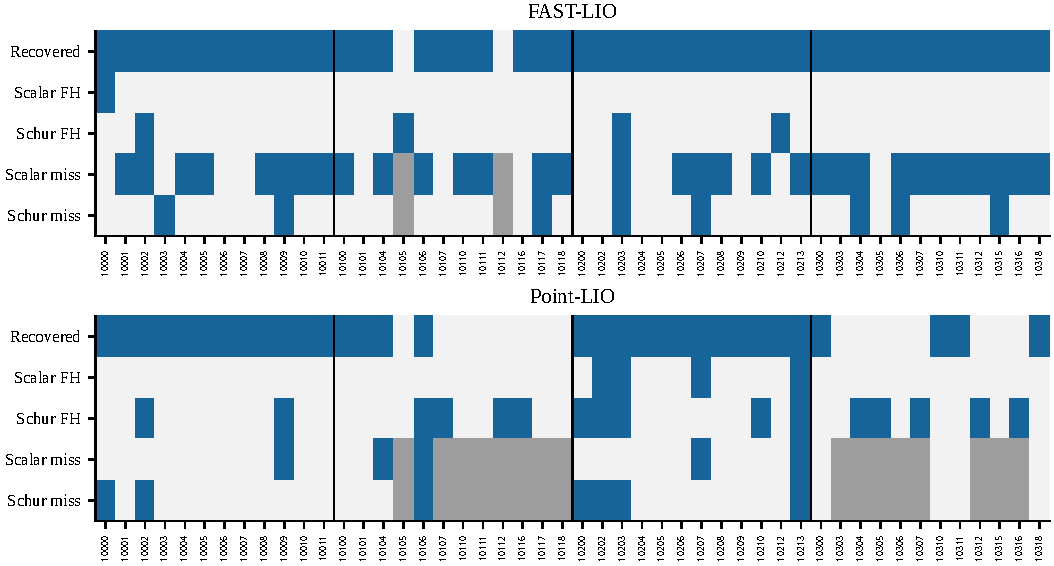
\includegraphics[width=\textwidth]{assets/all_event_ledger.pdf}
\caption{Complete event map from retained exports. Columns are the 48 selected seeds,
ordered within SN, SW, LN and LW groups. Dark blue marks a recovered event or a
present FH/missed-declaration event in its named row. Light cells mean absence;
grey cells are not applicable because reference recovery did not occur.
Policy-event rows are paired within geometry, not independent replicates.}\label{fig:all}
\end{figure}
\begingroup\footnotesize
\begin{longtable}{@{}llclllrl@{}}
\caption{FAST-LIO: all 96 policy-event rows (48 shared geometries; S = scalar, D = adapted directional rule).}\\
\toprule
Group & Seed & Policy & Truth & FH & Declared & Delay (s) & Miss class\\\midrule\endfirsthead
\multicolumn{8}{c}{\tablename\ \thetable{} -- continued}\\
\toprule
Group & Seed & Policy & Truth & FH & Declared & Delay (s) & Miss class\\\midrule\endhead
\midrule\multicolumn{8}{r}{Continued on next page}\\\endfoot
\bottomrule\endlastfoot
SN & 10000 & D & R & no & yes & 13.400 & --\\
SN & 10000 & S & R & yes & yes & 15.400 & --\\
SN & 10001 & D & R & no & yes & 13.600 & --\\
SN & 10001 & S & R & no & no & -- & raw\\
SN & 10002 & D & R & yes & yes & 12.900 & --\\
SN & 10002 & S & R & no & no & -- & raw\\
SN & 10003 & D & R & no & no & -- & raw\\
SN & 10003 & S & R & no & yes & 5.500 & --\\
SN & 10004 & D & R & no & yes & 12.300 & --\\
SN & 10004 & S & R & no & no & -- & raw\\
SN & 10005 & D & R & no & yes & 5.800 & --\\
SN & 10005 & S & R & no & no & -- & raw\\
SN & 10006 & D & R & no & yes & 13.300 & --\\
SN & 10006 & S & R & no & yes & 0.500 & --\\
SN & 10007 & D & R & no & yes & 6.000 & --\\
SN & 10007 & S & R & no & yes & 0.100 & --\\
SN & 10008 & D & R & no & yes & 8.500 & --\\
SN & 10008 & S & R & no & no & -- & raw\\
SN & 10009 & D & R & no & no & -- & raw\\
SN & 10009 & S & R & no & no & -- & raw\\
SN & 10010 & D & R & no & yes & 10.200 & --\\
SN & 10010 & S & R & no & no & -- & confirm\\
SN & 10011 & D & R & no & yes & 0.500 & --\\
SN & 10011 & S & R & no & no & -- & raw\\
SW & 10100 & D & R & no & yes & 12.100 & --\\
SW & 10100 & S & R & no & no & -- & raw\\
SW & 10101 & D & R & no & yes & 9.300 & --\\
SW & 10101 & S & R & no & yes & 0.900 & --\\
SW & 10104 & D & R & no & yes & 6.100 & --\\
SW & 10104 & S & R & no & no & -- & raw\\
SW & 10105 & D & NR & yes & no & -- & --\\
SW & 10105 & S & NR & no & no & -- & --\\
SW & 10106 & D & R & no & yes & 16.400 & --\\
SW & 10106 & S & R & no & no & -- & raw\\
SW & 10107 & D & R & no & yes & 13.800 & --\\
SW & 10107 & S & R & no & yes & 0.400 & --\\
SW & 10110 & D & R & no & yes & 10.200 & --\\
SW & 10110 & S & R & no & no & -- & raw\\
SW & 10111 & D & R & no & yes & 9.500 & --\\
SW & 10111 & S & R & no & no & -- & raw\\
SW & 10112 & D & NR & no & no & -- & --\\
SW & 10112 & S & NR & no & no & -- & --\\
SW & 10116 & D & R & no & yes & 13.900 & --\\
SW & 10116 & S & R & no & yes & 0.200 & --\\
SW & 10117 & D & R & no & no & -- & confirm\\
SW & 10117 & S & R & no & no & -- & raw\\
SW & 10118 & D & R & no & yes & 4.300 & --\\
SW & 10118 & S & R & no & no & -- & raw\\
LN & 10200 & D & R & no & yes & 1.200 & --\\
LN & 10200 & S & R & no & yes & 5.700 & --\\
LN & 10202 & D & R & no & yes & 1.100 & --\\
LN & 10202 & S & R & no & yes & 5.400 & --\\
LN & 10203 & D & R & yes & no & -- & active\\
LN & 10203 & S & R & no & no & -- & raw\\
LN & 10204 & D & R & no & yes & 0.900 & --\\
LN & 10204 & S & R & no & yes & 1.800 & --\\
LN & 10205 & D & R & no & yes & 0.200 & --\\
LN & 10205 & S & R & no & yes & 1.500 & --\\
LN & 10206 & D & R & no & yes & 7.500 & --\\
LN & 10206 & S & R & no & no & -- & raw\\
LN & 10207 & D & R & no & no & -- & confirm\\
LN & 10207 & S & R & no & no & -- & raw\\
LN & 10208 & D & R & no & yes & 3.400 & --\\
LN & 10208 & S & R & no & no & -- & raw\\
LN & 10209 & D & R & no & yes & 1.300 & --\\
LN & 10209 & S & R & no & yes & 0.800 & --\\
LN & 10210 & D & R & no & yes & 12.600 & --\\
LN & 10210 & S & R & no & no & -- & confirm\\
LN & 10212 & D & R & yes & yes & 17.800 & --\\
LN & 10212 & S & R & no & yes & 0.300 & --\\
LN & 10213 & D & R & no & yes & 0.800 & --\\
LN & 10213 & S & R & no & no & -- & raw\\
LW & 10300 & D & R & no & yes & 13.400 & --\\
LW & 10300 & S & R & no & no & -- & raw\\
LW & 10303 & D & R & no & yes & 8.900 & --\\
LW & 10303 & S & R & no & no & -- & raw\\
LW & 10304 & D & R & no & no & -- & raw\\
LW & 10304 & S & R & no & no & -- & raw\\
LW & 10305 & D & R & no & yes & 2.400 & --\\
LW & 10305 & S & R & no & yes & 0.000 & --\\
LW & 10306 & D & R & no & no & -- & raw\\
LW & 10306 & S & R & no & no & -- & raw\\
LW & 10307 & D & R & no & yes & 4.500 & --\\
LW & 10307 & S & R & no & no & -- & raw\\
LW & 10310 & D & R & no & yes & 1.800 & --\\
LW & 10310 & S & R & no & no & -- & raw\\
LW & 10311 & D & R & no & yes & 5.000 & --\\
LW & 10311 & S & R & no & no & -- & raw\\
LW & 10312 & D & R & no & yes & 4.000 & --\\
LW & 10312 & S & R & no & no & -- & raw\\
LW & 10315 & D & R & no & no & -- & raw\\
LW & 10315 & S & R & no & no & -- & raw\\
LW & 10316 & D & R & no & yes & 3.400 & --\\
LW & 10316 & S & R & no & no & -- & raw\\
LW & 10318 & D & R & no & yes & 5.400 & --\\
LW & 10318 & S & R & no & no & -- & raw\\
\end{longtable}\endgroup

\begingroup\footnotesize
\begin{longtable}{@{}llclllrl@{}}
\caption{Point-LIO: all 96 policy-event rows (48 shared geometries; S = scalar, D = adapted directional rule).}\\
\toprule
Group & Seed & Policy & Truth & FH & Declared & Delay (s) & Miss class\\\midrule\endfirsthead
\multicolumn{8}{c}{\tablename\ \thetable{} -- continued}\\
\toprule
Group & Seed & Policy & Truth & FH & Declared & Delay (s) & Miss class\\\midrule\endhead
\midrule\multicolumn{8}{r}{Continued on next page}\\\endfoot
\bottomrule\endlastfoot
SN & 10000 & D & R & no & no & -- & raw\\
SN & 10000 & S & R & no & yes & 5.000 & --\\
SN & 10001 & D & R & no & yes & 3.400 & --\\
SN & 10001 & S & R & no & yes & 4.900 & --\\
SN & 10002 & D & R & yes & no & -- & active\\
SN & 10002 & S & R & no & yes & 4.300 & --\\
SN & 10003 & D & R & no & yes & 11.800 & --\\
SN & 10003 & S & R & no & yes & 7.100 & --\\
SN & 10004 & D & R & no & yes & 3.300 & --\\
SN & 10004 & S & R & no & yes & 0.500 & --\\
SN & 10005 & D & R & no & yes & 3.200 & --\\
SN & 10005 & S & R & no & yes & 4.500 & --\\
SN & 10006 & D & R & no & yes & 11.700 & --\\
SN & 10006 & S & R & no & yes & 4.100 & --\\
SN & 10007 & D & R & no & yes & 0.000 & --\\
SN & 10007 & S & R & no & yes & 2.700 & --\\
SN & 10008 & D & R & no & yes & 7.800 & --\\
SN & 10008 & S & R & no & yes & 4.900 & --\\
SN & 10009 & D & R & yes & yes & 0.100 & --\\
SN & 10009 & S & R & no & no & -- & raw\\
SN & 10010 & D & R & no & yes & 2.200 & --\\
SN & 10010 & S & R & no & yes & 3.400 & --\\
SN & 10011 & D & R & no & yes & 0.000 & --\\
SN & 10011 & S & R & no & yes & 2.700 & --\\
SW & 10100 & D & R & no & yes & 3.200 & --\\
SW & 10100 & S & R & no & yes & 0.200 & --\\
SW & 10101 & D & R & no & yes & 10.400 & --\\
SW & 10101 & S & R & no & yes & 0.300 & --\\
SW & 10104 & D & R & no & yes & 1.200 & --\\
SW & 10104 & S & R & no & no & -- & raw\\
SW & 10105 & D & NR & no & no & -- & --\\
SW & 10105 & S & NR & no & no & -- & --\\
SW & 10106 & D & R & yes & no & -- & raw\\
SW & 10106 & S & R & no & no & -- & raw\\
SW & 10107 & D & NR & yes & no & -- & --\\
SW & 10107 & S & NR & no & no & -- & --\\
SW & 10110 & D & NR & no & no & -- & --\\
SW & 10110 & S & NR & no & no & -- & --\\
SW & 10111 & D & NR & no & no & -- & --\\
SW & 10111 & S & NR & no & no & -- & --\\
SW & 10112 & D & NR & yes & no & -- & --\\
SW & 10112 & S & NR & no & no & -- & --\\
SW & 10116 & D & NR & yes & no & -- & --\\
SW & 10116 & S & NR & no & no & -- & --\\
SW & 10117 & D & NR & no & no & -- & --\\
SW & 10117 & S & NR & no & no & -- & --\\
SW & 10118 & D & NR & no & no & -- & --\\
SW & 10118 & S & NR & no & no & -- & --\\
LN & 10200 & D & R & yes & no & -- & active\\
LN & 10200 & S & R & no & yes & 2.800 & --\\
LN & 10202 & D & R & yes & no & -- & active\\
LN & 10202 & S & R & yes & yes & 14.400 & --\\
LN & 10203 & D & R & yes & no & -- & active\\
LN & 10203 & S & R & yes & yes & 18.100 & --\\
LN & 10204 & D & R & no & yes & 0.700 & --\\
LN & 10204 & S & R & no & yes & 4.700 & --\\
LN & 10205 & D & R & no & yes & 10.700 & --\\
LN & 10205 & S & R & no & yes & 0.400 & --\\
LN & 10206 & D & R & no & yes & 0.500 & --\\
LN & 10206 & S & R & no & yes & 0.800 & --\\
LN & 10207 & D & R & no & yes & 7.900 & --\\
LN & 10207 & S & R & yes & no & -- & active\\
LN & 10208 & D & R & no & yes & 3.000 & --\\
LN & 10208 & S & R & no & yes & 0.300 & --\\
LN & 10209 & D & R & no & yes & 9.900 & --\\
LN & 10209 & S & R & no & yes & 0.100 & --\\
LN & 10210 & D & R & yes & yes & 0.300 & --\\
LN & 10210 & S & R & no & yes & 0.300 & --\\
LN & 10212 & D & R & no & yes & 11.500 & --\\
LN & 10212 & S & R & no & yes & 2.200 & --\\
LN & 10213 & D & R & yes & no & -- & active\\
LN & 10213 & S & R & yes & no & -- & active\\
LW & 10300 & D & R & no & yes & 2.700 & --\\
LW & 10300 & S & R & no & yes & 8.200 & --\\
LW & 10303 & D & NR & no & no & -- & --\\
LW & 10303 & S & NR & no & no & -- & --\\
LW & 10304 & D & NR & yes & no & -- & --\\
LW & 10304 & S & NR & no & no & -- & --\\
LW & 10305 & D & NR & yes & no & -- & --\\
LW & 10305 & S & NR & no & no & -- & --\\
LW & 10306 & D & NR & no & no & -- & --\\
LW & 10306 & S & NR & no & no & -- & --\\
LW & 10307 & D & NR & yes & no & -- & --\\
LW & 10307 & S & NR & no & no & -- & --\\
LW & 10310 & D & R & no & yes & 0.300 & --\\
LW & 10310 & S & R & no & yes & 4.200 & --\\
LW & 10311 & D & R & no & yes & 0.100 & --\\
LW & 10311 & S & R & no & yes & 2.500 & --\\
LW & 10312 & D & NR & yes & no & -- & --\\
LW & 10312 & S & NR & no & no & -- & --\\
LW & 10315 & D & NR & no & no & -- & --\\
LW & 10315 & S & NR & no & no & -- & --\\
LW & 10316 & D & NR & yes & no & -- & --\\
LW & 10316 & S & NR & no & no & -- & --\\
LW & 10318 & D & R & no & yes & 0.000 & --\\
LW & 10318 & S & R & no & yes & 15.200 & --\\
\end{longtable}\endgroup


\section{Machine-readable supporting files and reproduction}
The adjacent \texttt{support/} folder includes the full-precision diagnostic-event
ledger, exploratory diagnosis, all 64 screen candidates, all 192 native-run
receipts, native build identities, copied configurations, selected timeline
metadata and asset/source hashes. The full native ledger records backend,
seed, group, scene, run identity, completion status, exit code, elapsed time,
manifest digest and retained manifest path. Absolute original paths are provenance;
the portable reproduction package supplies a relocation map.

The versioned reproduction package is listed below with its verified repository commit.
\begin{lstlisting}
reproduction/lidar_recovery_20261023/
d696dab58d93bcd640e3651965246bf9158d2d0e
\end{lstlisting}
Its offline reanalysis regenerated 96 recovery labels, 192 event rows and
20 figures; discrete labels and decisions agreed exactly and maximum numerical
difference was $7.1\times10^{-15}$. The original 197-entry implementation freeze
remains separately verified. That check certifies the packaged offline reanalysis,
not a complete native estimator replay on another machine. Current source and
original frozen source are distinguished in the package.

The main manuscript and this supplement are drafts awaiting human author review,
verified affiliations and declarations, venue selection and its exact submission
requirements. Scientific review must assess comparator fidelity and whether this
bounded empirical contribution is sufficient for the chosen venue. These
materials support that review without promising publication acceptance.
\end{document}
